\headline{{\textbf{\Large\sffamily Bonsai Roots:}}\\
          {\textbf{\large\sffamily Meet the Members of TWBC}}}
\label{2025-03-roots}
\noindent
Welcome to the latest edition of \emph{Bonsai Roots}, our monthly column where we highlight the individuals who make up the heart of the Twickenham Bonsai Club.
This feature aims to deepen connections within our community and provide potential new members with a closer look at the people who shape our vibrant club.

This month, we're pleased to introduce \textbf{Mark Edwards}, a passionate bonsai enthusiast who has been steadily growing his collection.
Mark has been involved in bonsai for several years, but like many, his passion truly ignited during lockdown.
With a collection of around 30 trees and an appreciation for both rare maples and challenging pines, we're excited to learn more about Mark and his bonsai journey.

\begin{itemize}
    \item \textbf{What's your name and where in the country do you live?}
    
    \emph{My name is Mark Edwards, and I live in Hampton Wick, UK.}

    \item \textbf{What are your favourite species of tree and why?}
    
    \emph{Choosing a favourite is tough, but I'd have to say Japanese maples. I have a rare Arakawa and an even rarer Beni Chidori---both are my favourites.}

    \item \textbf{What aspect of bonsai do you enjoy?}
    
    \emph{I love old, established trees, but even my 80\--100\--year\--old maples require constant attention. All my trees are ongoing in their progression. I also really enjoy wiring.}

    \item \textbf{What aspects of bonsai do you find most challenging?}
    
    \emph{Pines! They are so different from deciduous trees, and I find them particularly challenging to work with.}

    \begin{window}[%
        2,l,%
        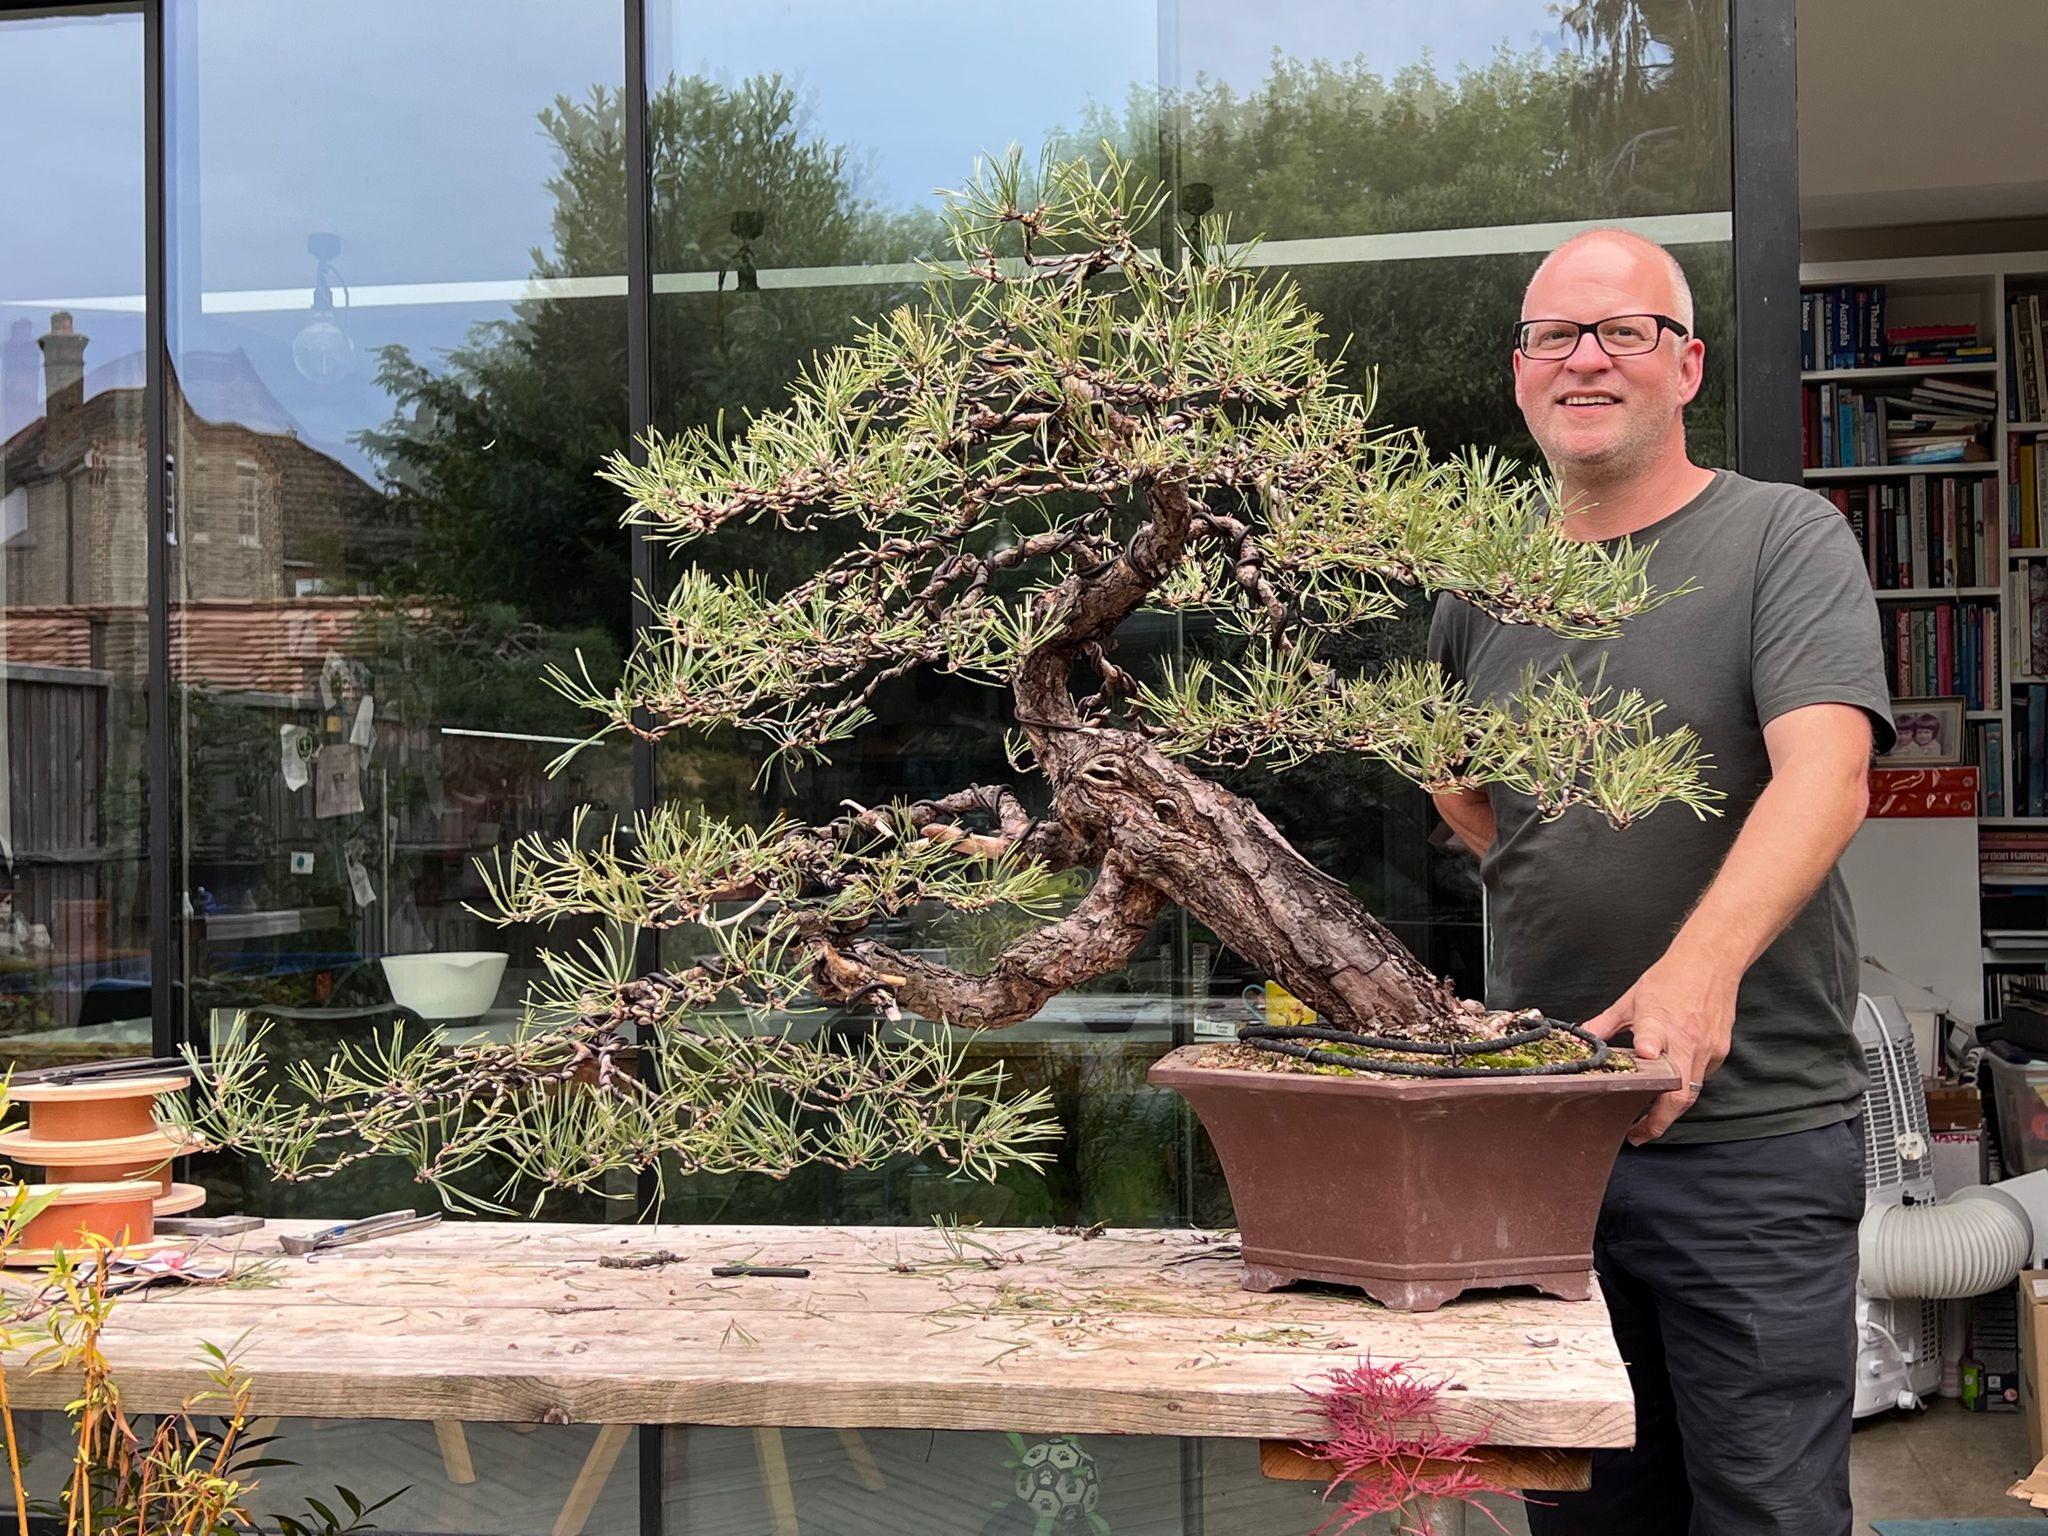
\includegraphics[width=1.0\columnwidth]{2025_03/res/roots_mark_edwards},%
        \centerline{\emph{Mark with his cherished Scots Pine, a tree with history.}}%
    ]
    \end{window}
    \columnbreak

    \item \textbf{Who or what inspires you throughout your bonsai journey?}
    
    \emph{I find inspiration from many people. I've had Nacho Salar over a few times, and more recently, Caz, who was both great fun and incredibly knowledgeable.}

    \item \textbf{How long have you been interested in bonsai?}
    
    \emph{I've been interested since I was a teenager, but my first trees didn't fare too well. About eight years ago, I bought a couple and still have those. Then, during lockdown, I really got into bonsai---it provided a sense of normality, and I could lose myself in learning about it.}

    \item \textbf{What stimulated your interest in bonsai?}
    
    \emph{I've always found bonsai beautiful, but what really captured me was the skill involved. I'm a model maker and hairdresser by trade, and bonsai is like a blend of those two worlds. Manipulating nature---it's crazy stuff!}

    \item \textbf{If you could give someone new to bonsai any tips, what would it be?}
    
    \emph{Be prepared for a steep learning curve. It's intense but incredibly rewarding. Don't be scared! I didn't start with sticks in pots---I went straight in with large, expensive trees, which meant I had to keep them alive because I'd invested so much into them! Also, invest in a greenhouse or polytunnel. I learnt the hard way and lost some beautiful trees during a particularly harsh winter.}

    \item \textbf{Why do you enjoy being part of TWBC, and do you have any ideas or suggestions for the club's future?}
    
    \emph{I haven't been the most active member since joining because my daughter was heavily involved in under-16 women's basketball, which kept me busy most Thursday evenings. However, I've enjoyed bouncing around ideas and advice with fellow members, and now that my daughter has given up basketball, I fully intend to be more involved.}

    \item \textbf{One word to describe what bonsai means to you?}
    
    \emph{Therapeutic.}

    \item \textbf{What are your future goals regarding your own trees and learning more about the hobby?}
    
    \emph{To improve all my trees as much as possible and to keep learning. Once you think you know it all, you may as well give up---there's always something new to discover.}

    \item \textbf{How would you like to see your bonsai journey progress in the future?}
    
    \emph{I'd love to see some of my trees at Chelsea, winning a medal.}
\end{itemize}

We hope you've enjoyed getting to know Mark and his bonsai journey.
Stay tuned to \emph{Bonsai Roots} for more member stories in the coming months!

\closearticle
